\documentclass[10pt]{article}
\usepackage[margin=0.8in]{geometry}
\usepackage[T1]{fontenc}
\usepackage{lmodern,hyperref,tikz}
\hypersetup{colorlinks=true,urlcolor=blue}
\setlength{\parindent}{0pt}\setlength{\parskip}{7pt}\sloppy
\begin{document}
\begin{center}{\LARGE Relation information and Kummer source contracts}\\[6pt]Source-only audit, 1 November 2026\end{center}
The audit identifies six composition contracts joining physical execution, signed labelled divisors, graph relations, target information and complete charged work. Existing implementations and review artifacts are reused. No experiments, new target trajectories, cloud actions, timing measurements or theorem certifications were performed.
\textbf{Scope preserved:} 1,260 targets. Complete cost ratio and natural yield remain null. This packet is a source-contract map, not a completion certificate.
\begin{center}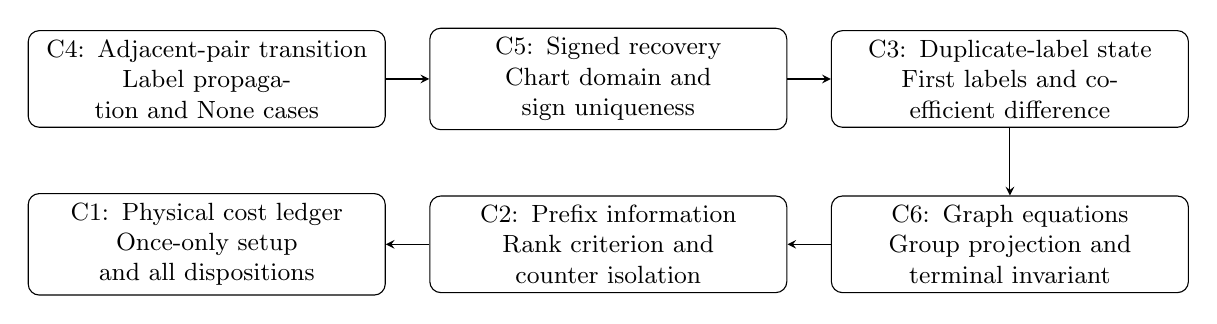
\begin{tikzpicture}[every node/.style={draw,rounded corners,text width=4.3cm,align=center,minimum height=1.1cm,font=\small},>=stealth]
\node (n0) at (0,0) {C4: Adjacent-pair transition\\Label propagation and None cases};
\node (n1) at (5.1,0) {C5: Signed recovery\\Chart domain and sign uniqueness};
\node (n2) at (10.2,0) {C3: Duplicate-label state\\First labels and coefficient difference};
\node (n3) at (10.2,-2.1) {C6: Graph equations\\Group projection and terminal invariant};
\node (n4) at (5.1,-2.1) {C2: Prefix information\\Rank criterion and counter isolation};
\node (n5) at (0,-2.1) {C1: Physical cost ledger\\Once-only setup and all dispositions};
\draw[->] (n0) -- (n1);
\draw[->] (n1) -- (n2);
\draw[->] (n2) -- (n3);
\draw[->] (n3) -- (n4);
\draw[->] (n4) -- (n5);
\end{tikzpicture}\end{center}
Arrows indicate required composition; a node does not assert that its obligation is proved. The editable SVG contains the same dependency sequence.
\textbf{Historical saved observations.} The prior portfolio inventory contained 140 files, all matching their recorded hashes during the preceding read-only audit. Its standardized table records five factor-base arms with 1,260 rows each, two law arms with 1,260 each and a Kummer differential arm with 1,260. Historical pencil coverage records 543 verified candidate keys, one capped-only key and 716 without indexed candidate rows. The later C1 gate records 7/18 observations, 4/15 measured, no complete pairs and two timeouts. These are saved-artifact counts, not new runs or scalar replays.
The retained duplicate archive analysis reports 420 dispositions: 218 ineligible and 202 compared, comprising 174 first observations and 28 redundant observations. The actual source uses retained coordinate witnesses, so these counts do not estimate naturally generated duplicate yield.
\newpage
\section*{C1-physical-cost-partition}
\textbf{Existing evidence.} archive\_target emits setup\_checks\_field and constructor\_field repeatedly for seven retained cases. Its explicit metadata says these copies are nonadditive and aggregate once per physical archive\_row. Analysis already groups setup by physical row and reports no consistency errors.
\textbf{Unproved or unbound transition.} No complete timing or cost denominator. Constructors contain Ring primality and allocation work outside field counters; input parsing, curve construction, hashing, memory, comparisons and square-root nonresidue search also need their own accounting. This is retained-coordinate input, not a naturally generated production stream.
\textbf{Concrete contract.} For immutable input archive hash H, let P=(H,archive\_row). Require exactly one setup and constructor record per P, identical repeated metadata, and one disposition per (P,case\_index). Total charged work is sum\_P setup(P)+constructor(P) plus all disjoint per-case intervals and declared run-global work. Never sum copied setup on each case; never equate target\_index with physical identity across archives. Preserve failure, skipped, poisoned and post-terminal dispositions with explicit charged/non-production reason.
\textbf{Next source/proof work.} Write schema-level bijection and disjoint-interval checker contract against existing ledger, not a replacement aggregate.
\textbf{Source references:} archive:855-881, archive\_entry:2, accounting.
\section*{C2-production-prefix-information}
\textbf{Existing evidence.} information computes rank(A), rank([A b]), rank([A b c]); consistent iff full rank equals augmented-target rank; target determined iff consistent and rank gain one. Adapter validates then normalizes and flips only final RHS column. Independent sign review exists.
\textbf{Unproved or unbound transition.} The diagnostic performs six rank computations through two information calls and mutates thread-local arithmetic counters. It has no production prefix completeness bridge, emitted-stream custody or policy experiment.
\textbf{Concrete contract.} For each production row identity, bind curve/target/ring, physical source event, accepted signed factors, source labels and exact augmented sign convention. Prefix export must be bijective with accepted preterminal events and preserve rejected/duplicate dispositions separately. Compute offline diagnostic after snapshotting production counters; either isolate diagnostic counters or account them as a distinct analysis phase. At each prefix target information is consistency AND rank([A b])-rank(A)=1, not total rank or cycle count.
\textbf{Next source/proof work.} Specify adapter for actual retained emitted prefixes and count boundary; reuse existing rank and sign routines.
\textbf{Source references:} information:34-56, adapter:1-26, adapter\_review.
\newpage
\section*{C3-duplicate-label-invariant}
\textbf{Existing evidence.} Signed coefficient-difference lemma and independent 12-case review exist. Native Labels stores first sign-normalized pair and suppresses duplicate graph edges. Candidate is verified against Q.
\textbf{Unproved or unbound transition.} Labels::ingest accepts D without checking validity or D=aG+bQ. Constructor checks rG=rQ=0 but not Q in <G>. Retained harness supplies the stronger equality with planted-scalar setup; prospective production must establish it from initialized and propagated labels.
\textbf{Concrete contract.} In fixed target context with ord(G)=prime r, Q=kG and D=aG+bQ, canonical key/sign must satisfy sigma D=C and both labels normalize by sigma. Preserve first pair unchanged. Equal keys imply delta\_a+delta\_b*k=0; db=0 forces da=0, else verified candidate is -da/db. Closure theorem must connect every actual transition to the label invariant; rQ=0 alone is not the subgroup premise.
\textbf{Next source/proof work.} Formalize native table-state preservation and caller-to-ingest label transport; do not redo the existing elementary duplicate lemma as if new.
\textbf{Source references:} duplicate:1-22, archive:863-879, lemma, lemma\_review.
\section*{C4-original-G-transition-closure}
\textbf{Existing evidence.} advance implements geometric step, optional validation, then signed fallback only if geometric step returns None. Original-G fixture has 63 transitions per arm and candidate63 exact recoveries.
\textbf{Unproved or unbound transition.} When validate\_transition=false and geometric step returns Some, no internal full signed validation executes. Finite fixture excludes successful repair and Delta-zero branches. Signed fallback can return None after validity/projection failure; thus universal total closure is not proved.
\textbf{Concrete contract.} Define Adj(k,kp,a,b): both nonzero valid Kummer representatives of D=aG+bQ and D+G, with canonical labels and rG=rQ=0. Under explicit projection/chart/repair domain, advance Some must preserve Adj at (2a+choice mod r,2b mod r); choice in \{0,1\}. Separately characterize every None and prove retry policy preserves target identity and charges abandoned work. Word arithmetic requires bound ensuring 2a+choice and 2b do not overflow (r$\le$2\textasciicircum{}63 suffices for a,b<r).
\textbf{Next source/proof work.} Prove source-return soundness branch by branch before claiming total closure; enumerate chart-domain predicates as preconditions rather than assuming fallback always succeeds.
\textbf{Source references:} transition:235-324, original\_status.
\newpage
\section*{C5-signed-lift-uniqueness}
\textbf{Existing evidence.} lift dispatches general recovery, D\_zero exceptional search, Delta\_zero lift and degree-one boundary lift. Boundary implementation filters candidate validity and two projective equalities and returns only a unique candidate.
\textbf{Unproved or unbound transition.} Kernel connection from projective equality to unique signed Jacobian value is not supplied by fixture counts. Ambiguous torsion anchors, invalid/singular charts and no-match outputs remain explicit cases.
\textbf{Concrete contract.} Given valid anchor G and neighbor pair (kappa(D),kappa(D+G)), prove each Some result equals D under the exact chart and sign-uniqueness assumptions; prove zero/ambiguous/no-match outputs are classified without treating projection equality alone as sign equality. General and exceptional implementations need separate source bindings; preserve actual nonsquare/singular failures.
\textbf{Next source/proof work.} Bind existing boundary and original-G reviews to precise sufficient uniqueness premises; prove one shared result interface across recovery branches.
\textbf{Source references:} transition:175-219, original\_status.
\section*{C6-graph-to-group-and-terminal}
\textbf{Existing evidence.} Graph adapter factors recovered split degree-two D, assigns canonical signs and checks factor sum in fixtures. Independent dense elimination checked emitted prefixes; synthetic terminal controls exist. Graph review explicitly reports zero geometric terminal returns.
\textbf{Unproved or unbound transition.} A compatible F\_r scalar coordinate for every factor-base point class is not established by ord(G)=r. Geometric graph terminal/duplicate/repeated-root branches were not exercised in that fixture. Verification-on-return is not a proof of target extraction completeness.
\textbf{Concrete contract.} Supply an actual homomorphism phi from the subgroup generated by all relevant divisor classes to F\_r with phi(G)=1 and phi(Q)=k, or restrict points to a justified subgroup/projection. Then prove every inserted su*Xu+sv*Xv=a+b*k row follows from D=aG+bQ and factor decomposition. Prove signed union-find potential invariant and that a nonzero eliminated target coefficient yields k; preserve zero-information cycles and consistency failures.
\textbf{Next source/proof work.} Identify the precise group-model/projection premise from existing construction and state the graph invariant against it; do not infer it from r-torsion tests.
\textbf{Source references:} graph:10-16, graph\_review, lemma.
\newpage
\section*{Accounting partition}
All intervals reflect the fixed retained harness. Production-vs-reference split needs frozen protocol; all actual incurred costs remain preserved.
\textbf{Physical identity:} (input\_archive\_sha256, physical\_archive\_row, case\_index)
\textbf{setup\_once}\begin{itemize}
\item setup\_checks\_field
\item constructor\_field
\end{itemize}
\textbf{per\_case\_disjoint}\begin{itemize}
\item label\_reference\_field
\item eligibility\_field
\item key\_reference\_field
\item adapter.field
\item adapter scalar\_after minus scalar\_before
\item graph.processing\_field
\item graph factor\_verification\_field
\item graph ring\_after minus ring\_before
\item terminal\_reference\_field
\end{itemize}
\textbf{nonadditive\_or\_external}\begin{itemize}
\item setup copies repeated on each case
\item graph state snapshots
\item walk/recovery custom counters may overlap field counts; require mapping before sums
\item dense reference work and offline rank work
\item host/runtime elapsed and memory not inferred from field counters
\end{itemize}
\section*{Source custody}
Exact absolute paths and SHA256 hashes are preserved in contracts.json. The following source keys bind the report statements.
\textbf{archive}: \nolinkurl{followup-continuation-v2/packets/retained-duplicate-executed/src/pruned.rs}\\{\scriptsize\texttt{e77db9e741da1d74b3dad97bf8f52c1128d4ac9e61eb0ea8dd62ddc923c21fcf}}\par
\textbf{archive\_entry}: \nolinkurl{followup-continuation-v2/packets/retained-duplicate-executed/src/check.rs}\\{\scriptsize\texttt{1f685079ab2ec640c271538db81b4a1d4a08fa7784424eeec07ba3efee636385}}\par
\textbf{duplicate}: \nolinkurl{followup-continuation-v2/packets/retained-duplicate-executed/src/duplicate.rs}\\{\scriptsize\texttt{33e74627a4b513b932e10b65f52fb5952ff8bc0473b3e0e76366689dc2494fd9}}\par
\textbf{accounting}: \nolinkurl{followup-continuation-v2/packets/retained-duplicate-executed/analysis.json}\\{\scriptsize\texttt{7024ed785cade871769b90a8d983a7e1828ccc59289c0f1225091a7a98f33fef}}\par
\textbf{graph}: \nolinkurl{followup-continuation-v2/packets/kummer-graph-integration/src/graph.rs}\\{\scriptsize\texttt{a612c5f4f2bea7c2573d147e4e54bfd2775fcf4057d2b11dd3ccf9cc63c58093}}\par
\textbf{transition}: \nolinkurl{followup-continuation-v2/packets/kummer-original-gstep/src/pruned.rs}\\{\scriptsize\texttt{149d55205b5edd872610350a2ddb7bf872d248f0e46f131b0091d618d33c6e5e}}\par
\textbf{lemma}: \nolinkurl{followup-continuation-v2/packets/kummer-target-rank/LEMMA.md}\\{\scriptsize\texttt{2a0d9c3a61941e6a066213e32890a0f5416098cc5b97f13dcbe0d5e23be83a20}}\par
\textbf{lemma\_review}: \nolinkurl{followup-continuation-v2/packets/kummer-target-rank-review/status.json}\\{\scriptsize\texttt{38eaf142ca7e732b7759c47d28b6f19be783a61c2e24bc64b488243b9e01955b}}\par
\textbf{graph\_review}: \nolinkurl{followup-continuation-v2/packets/kummer-graph-review/REVIEW.md}\\{\scriptsize\texttt{4830a8ec0a321a070fbddc5adb20cde532d824d5417643edc9bb54f9d261a236}}\par
\textbf{adapter}: \nolinkurl{followup-continuation-v2/relation-adapter/src/lib.rs}\\{\scriptsize\texttt{5c576f9675df206f463dee8169b860876b98c618f51b406323a35c7ed8423120}}\par
\textbf{adapter\_review}: \nolinkurl{followup-continuation-v2/packets/relation-adapter-review/REVIEW.md}\\{\scriptsize\texttt{d647ec25ae718a2c87dcbebf0b471162cef146b6a4f7bf4fcac7261484af70bf}}\par
\textbf{information}: \nolinkurl{five-followups/rank-information/src/lib.rs}\\{\scriptsize\texttt{602b0ebc368df64b3fdc019c3d2fed05ce3f12d437c8d297d4a8af3a37911f68}}\par
\textbf{original\_status}: \nolinkurl{followup-continuation-v2/packets/kummer-original-gstep/status.json}\\{\scriptsize\texttt{9c209baec29d03c45855f24fdb305ad32a9f236af213483c7f9916abeca29b70}}\par
\textbf{duplicate\_status}: \nolinkurl{followup-continuation-v2/packets/kummer-duplicate-adapter/status.json}\\{\scriptsize\texttt{9d18f55aec8d72f817da624cdd3d9ba6e7e578380eceae5d02eefe9d4f439d38}}\par
\end{document}
